\documentclass[10pt,a4paper]{report}
\usepackage[utf8]{inputenc}
\usepackage{amsmath}
\usepackage{amsfonts}
\usepackage{amssymb}
\usepackage{graphicx}
\usepackage[left=2cm,right=2cm,top=2cm,bottom=2cm]{geometry}
\begin{document}
\section{Background of Artray camera interaction}
The software package is based on the SDK provided freely by Artray in C\#, specifically on the CS.NET\_Graphic example software. 

\paragraph{Raw Artray data output}\label{sec:artrayRawOutput}
Data is handled and saved as one dimensional byte arrays by the SDK and has to be processed into a workable format.  The camera specifications allow for a maximum bit depth of 12 bit. To be able to access this bit depth the video format of "Color 48bit *" has to be set, as the monochrome formats do not allow higher bit depth. The single pixel data for the "Color 48bit *" setting is encoded as 2 byte per colour channel per pixel. Since, even though this is a monochrome camera, the colour output was not the same colour values for all returned subpixel types, meaning RGB, the saturation of the camera was set to be minimal in software (-255). This leads to identical red, green and blue subpixel values. From these 3 colour values, the first entry is arbitrarily chosen for further processing.
The data formatting is explained with the help of fig. \ref{fig:ByteArtrayOut}. Both bytes are formatted as big endian or most significant bit first. The second byte holds the most significant bit, with the first hex value and thus 4 bits being empty. The first byte holds the remaining 8 bits of the 12 bit value.

\begin{figure}[hbtp]
\centering
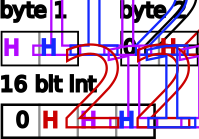
\includegraphics[scale=1]{images/ArtrayByteImage.png}
\caption{Data scheme of periodic byte structure of artray output with hexadecimal placeholders.\\
$\mathrm{H_{22}}$ holds the 4 most significant bit and byte 1 is simply appended.\\
$\mathrm{0_{21}}$ of byte 2 is always empty.\label{fig:ByteArtrayOut}}
\end{figure}

The value process via bitwise operations is then assigned to a short integer array. Saving of data is handled by a dialogue given by Artray dll to assure writing of correct raw data and thus cannot be directly influenced. This is the reason dimensions and position of region of interest saved have to be noted manually so far. Note that for processing the region of interest (ROI) needs to be known. It is not included in any of the raw data itself.
\end{document}